
%% bare_jrnl.tex
%% V1.4a
%% 2014/09/17
%% by Michael Shell
%% see http://www.michaelshell.org/
%% for current contact information.
%%
%% This is a skeleton file demonstrating the use of IEEEtran.cls
%% (requires IEEEtran.cls version 1.8a or later) with an IEEE
%% journal paper.
%%
%% Support sites:
%% http://www.michaelshell.org/tex/ieeetran/
%% http://www.ctan.org/tex-archive/macros/latex/contrib/IEEEtran/
%% and
%% http://www.ieee.org/

%%*************************************************************************
%% Legal Notice:
%% This code is offered as-is without any warranty either expressed or
%% implied; without even the implied warranty of MERCHANTABILITY or
%% FITNESS FOR A PARTICULAR PURPOSE! 
%% User assumes all risk.
%% In no event shall IEEE or any contributor to this code be liable for
%% any damages or losses, including, but not limited to, incidental,
%% consequential, or any other damages, resulting from the use or misuse
%% of any information contained here.
%%
%% All comments are the opinions of their respective authors and are not
%% necessarily endorsed by the IEEE.
%%
%% This work is distributed under the LaTeX Project Public License (LPPL)
%% ( http://www.latex-project.org/ ) version 1.3, and may be freely used,
%% distributed and modified. A copy of the LPPL, version 1.3, is included
%% in the base LaTeX documentation of all distributions of LaTeX released
%% 2003/12/01 or later.
%% Retain all contribution notices and credits.
%% ** Modified files should be clearly indicated as such, including  **
%% ** renaming them and changing author support contact information. **
%%
%% File list of work: IEEEtran.cls, IEEEtran_HOWTO.pdf, bare_adv.tex,
%%                    bare_conf.tex, bare_jrnl.tex, bare_conf_compsoc.tex,
%%                    bare_jrnl_compsoc.tex, bare_jrnl_transmag.tex
%%*************************************************************************


% *** Authors should verify (and, if needed, correct) their LaTeX system  ***
% *** with the testflow diagnostic prior to trusting their LaTeX platform ***
% *** with production work. IEEE's font choices and paper sizes can       ***
% *** trigger bugs that do not appear when using other class files.       ***                          ***
% The testflow support page is at:
% http://www.michaelshell.org/tex/testflow/



\documentclass[journal]{IEEEtran}
%
% If IEEEtran.cls has not been installed into the LaTeX system files,
% manually specify the path to it like:
% \documentclass[journal]{../sty/IEEEtran}





% Some very useful LaTeX packages include:
% (uncomment the ones you want to load)


% *** MISC UTILITY PACKAGES ***
%
%\usepackage{ifpdf}
% Heiko Oberdiek's ifpdf.sty is very useful if you need conditional
% compilation based on whether the output is pdf or dvi.
% usage:
% \ifpdf
%   % pdf code
% \else
%   % dvi code
% \fi
% The latest version of ifpdf.sty can be obtained from:
% http://www.ctan.org/tex-archive/macros/latex/contrib/oberdiek/
% Also, note that IEEEtran.cls V1.7 and later provides a builtin
% \ifCLASSINFOpdf conditional that works the same way.
% When switching from latex to pdflatex and vice-versa, the compiler may
% have to be run twice to clear warning/error messages.






% *** CITATION PACKAGES ***
%
%\usepackage{cite}
% cite.sty was written by Donald Arseneau
% V1.6 and later of IEEEtran pre-defines the format of the cite.sty package
% \cite{} output to follow that of IEEE. Loading the cite package will
% result in citation numbers being automatically sorted and properly
% "compressed/ranged". e.g., [1], [9], [2], [7], [5], [6] without using
% cite.sty will become [1], [2], [5]--[7], [9] using cite.sty. cite.sty's
% \cite will automatically add leading space, if needed. Use cite.sty's
% noadjust option (cite.sty V3.8 and later) if you want to turn this off
% such as if a citation ever needs to be enclosed in parenthesis.
% cite.sty is already installed on most LaTeX systems. Be sure and use
% version 5.0 (2009-03-20) and later if using hyperref.sty.
% The latest version can be obtained at:
% http://www.ctan.org/tex-archive/macros/latex/contrib/cite/
% The documentation is contained in the cite.sty file itself.






% *** GRAPHICS RELATED PACKAGES ***
%
\ifCLASSINFOpdf
   \usepackage[pdftex]{graphicx}
  % declare the path(s) where your graphic files are
  % \graphicspath{{../pdf/}{../jpeg/}}
  % and their extensions so you won't have to specify these with
  % every instance of \includegraphics
  % \DeclareGraphicsExtensions{.pdf,.jpeg,.png}
\else
  % or other class option (dvipsone, dvipdf, if not using dvips). graphicx
  % will default to the driver specified in the system graphics.cfg if no
  % driver is specified.
  % \usepackage[dvips]{graphicx}
  % declare the path(s) where your graphic files are
  % \graphicspath{{../eps/}}
  % and their extensions so you won't have to specify these with
  % every instance of \includegraphics
  % \DeclareGraphicsExtensions{.eps}
\fi
% graphicx was written by David Carlisle and Sebastian Rahtz. It is
% required if you want graphics, photos, etc. graphicx.sty is already
% installed on most LaTeX systems. The latest version and documentation
% can be obtained at: 
% http://www.ctan.org/tex-archive/macros/latex/required/graphics/
% Another good source of documentation is "Using Imported Graphics in
% LaTeX2e" by Keith Reckdahl which can be found at:
% http://www.ctan.org/tex-archive/info/epslatex/
%
% latex, and pdflatex in dvi mode, support graphics in encapsulated
% postscript (.eps) format. pdflatex in pdf mode supports graphics
% in .pdf, .jpeg, .png and .mps (metapost) formats. Users should ensure
% that all non-photo figures use a vector format (.eps, .pdf, .mps) and
% not a bitmapped formats (.jpeg, .png). IEEE frowns on bitmapped formats
% which can result in "jaggedy"/blurry rendering of lines and letters as
% well as large increases in file sizes.
%
% You can find documentation about the pdfTeX application at:
% http://www.tug.org/applications/pdftex





% *** MATH PACKAGES ***
%
\usepackage[cmex10]{amsmath}
% A popular package from the American Mathematical Society that provides
% many useful and powerful commands for dealing with mathematics. If using
% it, be sure to load this package with the cmex10 option to ensure that
% only type 1 fonts will utilized at all point sizes. Without this option,
% it is possible that some math symbols, particularly those within
% footnotes, will be rendered in bitmap form which will result in a
% document that can not be IEEE Xplore compliant!
%
% Also, note that the amsmath package sets \interdisplaylinepenalty to 10000
% thus preventing page breaks from occurring within multiline equations. Use:
%\interdisplaylinepenalty=2500
% after loading amsmath to restore such page breaks as IEEEtran.cls normally
% does. amsmath.sty is already installed on most LaTeX systems. The latest
% version and documentation can be obtained at:
% http://www.ctan.org/tex-archive/macros/latex/required/amslatex/math/





% *** SPECIALIZED LIST PACKAGES ***
%
%\usepackage{algorithmic}
% algorithmic.sty was written by Peter Williams and Rogerio Brito.
% This package provides an algorithmic environment fo describing algorithms.
% You can use the algorithmic environment in-text or within a figure
% environment to provide for a floating algorithm. Do NOT use the algorithm
% floating environment provided by algorithm.sty (by the same authors) or
% algorithm2e.sty (by Christophe Fiorio) as IEEE does not use dedicated
% algorithm float types and packages that provide these will not provide
% correct IEEE style captions. The latest version and documentation of
% algorithmic.sty can be obtained at:
% http://www.ctan.org/tex-archive/macros/latex/contrib/algorithms/
% There is also a support site at:
% http://algorithms.berlios.de/index.html
% Also of interest may be the (relatively newer and more customizable)
% algorithmicx.sty package by Szasz Janos:
% http://www.ctan.org/tex-archive/macros/latex/contrib/algorithmicx/




% *** ALIGNMENT PACKAGES ***
%
%\usepackage{array}
% Frank Mittelbach's and David Carlisle's array.sty patches and improves
% the standard LaTeX2e array and tabular environments to provide better
% appearance and additional user controls. As the default LaTeX2e table
% generation code is lacking to the point of almost being broken with
% respect to the quality of the end results, all users are strongly
% advised to use an enhanced (at the very least that provided by array.sty)
% set of table tools. array.sty is already installed on most systems. The
% latest version and documentation can be obtained at:
% http://www.ctan.org/tex-archive/macros/latex/required/tools/


% IEEEtran contains the IEEEeqnarray family of commands that can be used to
% generate multiline equations as well as matrices, tables, etc., of high
% quality.




% *** SUBFIGURE PACKAGES ***
%\ifCLASSOPTIONcompsoc
%  \usepackage[caption=false,font=normalsize,labelfont=sf,textfont=sf]{subfig}
%\else
  \usepackage[caption=false,font=footnotesize]{subfig}
%\fi
% subfig.sty, written by Steven Douglas Cochran, is the modern replacement
% for subfigure.sty, the latter of which is no longer maintained and is
% incompatible with some LaTeX packages including fixltx2e. However,
% subfig.sty requires and automatically loads Axel Sommerfeldt's caption.sty
% which will override IEEEtran.cls' handling of captions and this will result
% in non-IEEE style figure/table captions. To prevent this problem, be sure
% and invoke subfig.sty's "caption=false" package option (available since
% subfig.sty version 1.3, 2005/06/28) as this is will preserve IEEEtran.cls
% handling of captions.
% Note that the Computer Society format requires a larger sans serif font
% than the serif footnote size font used in traditional IEEE formatting
% and thus the need to invoke different subfig.sty package options depending
% on whether compsoc mode has been enabled.
%
% The latest version and documentation of subfig.sty can be obtained at:
% http://www.ctan.org/tex-archive/macros/latex/contrib/subfig/




% *** FLOAT PACKAGES ***
%
%\usepackage{fixltx2e}
% fixltx2e, the successor to the earlier fix2col.sty, was written by
% Frank Mittelbach and David Carlisle. This package corrects a few problems
% in the LaTeX2e kernel, the most notable of which is that in current
% LaTeX2e releases, the ordering of single and double column floats is not
% guaranteed to be preserved. Thus, an unpatched LaTeX2e can allow a
% single column figure to be placed prior to an earlier double column
% figure. The latest version and documentation can be found at:
% http://www.ctan.org/tex-archive/macros/latex/base/


%\usepackage{stfloats}
% stfloats.sty was written by Sigitas Tolusis. This package gives LaTeX2e
% the ability to do double column floats at the bottom of the page as well
% as the top. (e.g., "\begin{figure*}[!b]" is not normally possible in
% LaTeX2e). It also provides a command:
%\fnbelowfloat
% to enable the placement of footnotes below bottom floats (the standard
% LaTeX2e kernel puts them above bottom floats). This is an invasive package
% which rewrites many portions of the LaTeX2e float routines. It may not work
% with other packages that modify the LaTeX2e float routines. The latest
% version and documentation can be obtained at:
% http://www.ctan.org/tex-archive/macros/latex/contrib/sttools/
% Do not use the stfloats baselinefloat ability as IEEE does not allow
% \baselineskip to stretch. Authors submitting work to the IEEE should note
% that IEEE rarely uses double column equations and that authors should try
% to avoid such use. Do not be tempted to use the cuted.sty or midfloat.sty
% packages (also by Sigitas Tolusis) as IEEE does not format its papers in
% such ways.
% Do not attempt to use stfloats with fixltx2e as they are incompatible.
% Instead, use Morten Hogholm'a dblfloatfix which combines the features
% of both fixltx2e and stfloats:
%
% \usepackage{dblfloatfix}
% The latest version can be found at:
% http://www.ctan.org/tex-archive/macros/latex/contrib/dblfloatfix/




%\ifCLASSOPTIONcaptionsoff
%  \usepackage[nomarkers]{endfloat}
% \let\MYoriglatexcaption\caption
% \renewcommand{\caption}[2][\relax]{\MYoriglatexcaption[#2]{#2}}
%\fi
% endfloat.sty was written by James Darrell McCauley, Jeff Goldberg and 
% Axel Sommerfeldt. This package may be useful when used in conjunction with 
% IEEEtran.cls'  captionsoff option. Some IEEE journals/societies require that
% submissions have lists of figures/tables at the end of the paper and that
% figures/tables without any captions are placed on a page by themselves at
% the end of the document. If needed, the draftcls IEEEtran class option or
% \CLASSINPUTbaselinestretch interface can be used to increase the line
% spacing as well. Be sure and use the nomarkers option of endfloat to
% prevent endfloat from "marking" where the figures would have been placed
% in the text. The two hack lines of code above are a slight modification of
% that suggested by in the endfloat docs (section 8.4.1) to ensure that
% the full captions always appear in the list of figures/tables - even if
% the user used the short optional argument of \caption[]{}.
% IEEE papers do not typically make use of \caption[]'s optional argument,
% so this should not be an issue. A similar trick can be used to disable
% captions of packages such as subfig.sty that lack options to turn off
% the subcaptions:
% For subfig.sty:
% \let\MYorigsubfloat\subfloat
% \renewcommand{\subfloat}[2][\relax]{\MYorigsubfloat[]{#2}}
% However, the above trick will not work if both optional arguments of
% the \subfloat command are used. Furthermore, there needs to be a
% description of each subfigure *somewhere* and endfloat does not add
% subfigure captions to its list of figures. Thus, the best approach is to
% avoid the use of subfigure captions (many IEEE journals avoid them anyway)
% and instead reference/explain all the subfigures within the main caption.
% The latest version of endfloat.sty and its documentation can obtained at:
% http://www.ctan.org/tex-archive/macros/latex/contrib/endfloat/
%
% The IEEEtran \ifCLASSOPTIONcaptionsoff conditional can also be used
% later in the document, say, to conditionally put the References on a 
% page by themselves.




% *** PDF, URL AND HYPERLINK PACKAGES ***
%
%\usepackage{url}
% url.sty was written by Donald Arseneau. It provides better support for
% handling and breaking URLs. url.sty is already installed on most LaTeX
% systems. The latest version and documentation can be obtained at:
% http://www.ctan.org/tex-archive/macros/latex/contrib/url/
% Basically, \url{my_url_here}.




% *** Do not adjust lengths that control margins, column widths, etc. ***
% *** Do not use packages that alter fonts (such as pslatex).         ***
% There should be no need to do such things with IEEEtran.cls V1.6 and later.
% (Unless specifically asked to do so by the journal or conference you plan
% to submit to, of course. )


% correct bad hyphenation here
\hyphenation{op-tical net-works semi-conduc-tor}


\begin{document}
%
% paper title
% Titles are generally capitalized except for words such as a, an, and, as,
% at, but, by, for, in, nor, of, on, or, the, to and up, which are usually
% not capitalized unless they are the first or last word of the title.
% Linebreaks \\ can be used within to get better formatting as desired.
% Do not put math or special symbols in the title.
\title{Segmentation and Track-analysis in Time-lapse Imaging of Bacteria}
%
%
% author names and IEEE memberships
% note positions of commas and nonbreaking spaces ( ~ ) LaTeX will not break
% a structure at a ~ so this keeps an author's name from being broken across
% two lines.
% use \thanks{} to gain access to the first footnote area
% a separate \thanks must be used for each paragraph as LaTeX2e's \thanks
% was not built to handle multiple paragraphs
%

\author{Sajith~Kecheril~Sadanandan*,
		\"Ozden~Baltekin,        
        Klas~E.~G.~Magnusson,~\IEEEmembership{Student member,~IEEE, }% <-this % stops a space
		Alexis~Baucharin,
		Petter~Ranefall,
		Joakim~Jald\'en,~\IEEEmembership{Senior member,~IEEE,}
		Johan~Elf,
		Carolina~W\"ahlby,~\IEEEmembership{Senior member,~IEEE,}
\thanks{S. K. Sadanandan, P.~Ranefall and C.~W\"ahlby  are with the Department
of Information Technology, Uppsala University, Sweden and SciLifeLab, Sweden. C.~W\"ahlby is also with Broad Institute of Harvard and MIT, Cambridge, MA, USA.
e-mail: sajith.ks@it.uu.se}% <-this % stops a space
\thanks{A. Baucharin, \"O. Baltekin and J.~Elf are with the Department of Cell and Molecular Biology, Computational and Systems Biology, Uppsala University, Sweden }
\thanks{K. E. G. Magnusson and J. Jald\'en are with ACCESS Linnaeus Centre, KTH Royal Institute of Technology, Stockholm, Sweden }}% <-this % stops a space

%\thanks{Manuscript received April 19, 2005; revised September 17, 2014.}}

% note the % following the last \IEEEmembership and also \thanks - 
% these prevent an unwanted space from occurring between the last author name
% and the end of the author line. i.e., if you had this:
% 
% \author{....lastname \thanks{...} \thanks{...} }
%                     ^------------^------------^----Do not want these spaces!
%
% a space would be appended to the last name and could cause every name on that
% line to be shifted left slightly. This is one of those "LaTeX things". For
% instance, "\textbf{A} \textbf{B}" will typeset as "A B" not "AB". To get
% "AB" then you have to do: "\textbf{A}\textbf{B}"
% \thanks is no different in this regard, so shield the last } of each \thanks
% that ends a line with a % and do not let a space in before the next \thanks.
% Spaces after \IEEEmembership other than the last one are OK (and needed) as
% you are supposed to have spaces between the names. For what it is worth,
% this is a minor point as most people would not even notice if the said evil
% space somehow managed to creep in.



% The paper headers
%\markboth{Journal of \LaTeX\ Class Files,~Vol.~13, No.~9, September~2014}%
%{Shell \MakeLowercase{\textit{et al.}}: Bare Demo of IEEEtran.cls for Journals}
% The only time the second header will appear is for the odd numbered pages
% after the title page when using the twoside option.
% 
% *** Note that you probably will NOT want to include the author's ***
% *** name in the headers of peer review papers.                   ***
% You can use \ifCLASSOPTIONpeerreview for conditional compilation here if
% you desire.




% If you want to put a publisher's ID mark on the page you can do it like
% this:
%\IEEEpubid{0000--0000/00\$00.00~\copyright~2014 IEEE}
% Remember, if you use this you must call \IEEEpubidadjcol in the second
% column for its text to clear the IEEEpubid mark.



% use for special paper notices
%\IEEEspecialpapernotice{(Invited Paper)}




% make the title area
\maketitle

% As a general rule, do not put math, special symbols or citations
% in the abstract or keywords.
\begin{abstract}
Genetically identical cells express their genes at different levels and respond differently to changes in their environment.  Large-scale microscopy-based experiments are needed to characterize the dynamics of such cell-to-cell variability as well as the phenotypic diversity in response to perturbations in growth conditions. The rich data from image-based experiments requires robust and efficient analysis. In this work, we have developed tools to analyze bacterial cells growing in monolayers in a microfluidic device. Individual cells are identified using a novel curvature based approach and tracked over time for several generations. The resulting tracks are thereafter assessed and filtered based on track quality for subsequent analysis of bacterial growth rates. The proposed method performs better than the state-of-the-art methods for segmenting phase contrast and fluorescent images, and we show a 10-fold increase in analysis speed.
\end{abstract}

% Note that keywords are not normally used for peerreview papers.
\begin{IEEEkeywords}
E. coli, segmentation, time-lapse, microscopy, tracking.
\end{IEEEkeywords}






% For peer review papers, you can put extra information on the cover
% page as needed:
% \ifCLASSOPTIONpeerreview
% \begin{center} \bfseries EDICS Category: 3-BBND \end{center}
% \fi
%
% For peerreview papers, this IEEEtran command inserts a page break and
% creates the second title. It will be ignored for other modes.
\IEEEpeerreviewmaketitle



\section{Introduction}
% The very first letter is a 2 line initial drop letter followed
% by the rest of the first word in caps.
% 
% form to use if the first word consists of a single letter:
% \IEEEPARstart{A}{demo} file is ....
% 
% form to use if you need the single drop letter followed by
% normal text (unknown if ever used by IEEE):
% \IEEEPARstart{A}{}demo file is ....
% 
% Some journals put the first two words in caps:
% \IEEEPARstart{T}{his demo} file is ....
% 
% Here we have the typical use of a "T" for an initial drop letter
% and "HIS" in caps to complete the first word.
\IEEEPARstart{L}{ive} cell experiments pave the way to understand the complex biological functions of living organisms. Many live cell experiments require monitoring of cells under different conditions over several generations. Isogenic cells display cell-to-cell variability even when grown under similar conditions \cite{elowitzstochastic2002}. To study the origin and consequences of such variation it is necessary to monitor many individual cells for extended periods of time to reach statistically testable conclusions \cite{yuichiquantify2010}. Time-lapse experiments usually generate large quantities of data, which become extremely difficult for human observers to evaluate in an unbiased way \cite{qiangmicroscope2008}. Thus, automated systems are necessary to analyze such datasets in order to reach robust and reproducible results. 

Time-lapse imaging of growing bacterial cells are important both to answer fundamental biological questions related to the bacterial cell cycle as well as to study response to changes in growth condition due to changes in nutrients or antibiotics \cite{walldenstudying2011}. Based on the growth conditions and imaging modalities, various automated image segmentation and tracking packages were developed. For example \textit{MicrobeTracker} \cite {sliusarenkohigh2011} was designed to segment phase contrast images and detect fluorescent spots in a parallel fluorescent channel in bacterial cells grown isolated or in micro-colonies on agarose pads. \textit{Schnitzcells} \cite{youngmeasuring2012} was specifically designed to analyze fluorescent time-lapse images of \textit{E. coli} grown on agarose, and \textit{MAMLE} \cite {chowdhurycell2013} was designed to analyze \textit{E. coli} from phase contrast and fluorescent images.

Most image segmentation methods rely on raw pixel intensities to get an initial segmentation result, and further refined segmentation depends on this initial segmentation. \textit{MicrobeTracker} finds an initial segmentation using Otsu's thresholding method \cite {otsuthreshold1979} followed by edge detection and watershed segmentation. In the final step, active contours are applied to refine object boundaries. \textit{MicrobeTracker} needs manual correction of the first frame to get satisfactory segmentation results for time-lapse images. It is difficult to analyze large image sequences in \textit{MicrobeTracker} due to its inherent memory problems, and it is often necessary to modify the code for practical applications. \textit{MAMLE} uses range filtering to find an initial segmentation result, followed by multi-scale edge detection and a maximum likelihood classification to correct over- and under- segmentation. In \textit{Schnitzcells}, initial segmentation is achieved by edge detection followed by post processing to correct segmentation errors. 

Phase contrast images of \textit{E. coli} exhibit high-intensity regions inside cellular regions comparable to, or even brighter than, regions between cells. Relying on raw intensity therefore leads to over- and under-segmentation at the same time. The problem is amplified when trying to track cells over time. Even a $1\%$ error in detection of cells in every frame renders a cell lineage useless for further analysis if many cells are tracked over a long time.

Previously published cell tracking algorithms rely on model evolution, where a model of the cell is evolved over time using techniques such as active contour models \cite {zimmersegmentation2002} or level sets \cite {dzyubachykadvanced2010}, and tracking by detection \cite {bisereliable2011}. Tracking by detection involves two stages; segmentation and tracking. Sometimes both these steps are combined together to get a final tracking result \cite {jugoptimal2014}. 

In this work, we use tracking by detection, i.e., separate the segmentation and tracking problems and solve them separately, followed by a quality control and refinement step where some of the segmentation and tracking errors are corrected. Cell segmentation is done using our novel Curvature Based Approach, hereafter called as CBA, and tracking is done using a state-of-the-art tracking algorithm \cite {magnussonglobal2014}. In the following sections we present our segmentation methodology and compare it with that of \textit{MicrobeTracker} and \textit{MAMLE} on phase contrast as well as fluorescence images, from our own and previously published experiments. After segmentation, we track the cells through the time-lapse sequence and perform post tracking segmentation correction to get a final segmentation result. Finally, we show how the combined segmentation and tracking approach can be applied to quantify differences in cell growth rate under different experimental conditions.

\section{Methodology}
\subsection{Image Acquisition}
The bacterial cell colonies in our own experiments were grown on a specially designed microfluidic device in Polydimethylsiloxane(PDMS)\cite {ullmanhigh2012} with a growth chamber, a “trap”, of size $40 \times 40 \times 0.9\mu m$, which is open to growth media exchange at two ends.  The cells grow in a single layer and as the size of the microcolony gets larger than the trap, excess cells leave the trap through the outlet, thus maintaining the colony size of approximately $200$ cells nearly constant throughout the experiment. Images were captured using an inverted microscope fitted with separate cameras for phase contrast and fluorescent channels. The microscope was equipped with a TIR based hardware autofocus that keeps the cells in focus over days. $51$ traps can be monitored in parallel and growth conditions can be changed in $2$ seconds \cite{hammarlac2012} using computer controlled pumps. Phase contrast images were acquired every $30$ seconds at $125 ms$ exposure time using CFW-1312M (Scion Corporation) and fluorescent images were acquired every $60$ seconds using an EMCCD camera (Andor Technologies) and DPSS laser excitation at $514 nm$ (Coherent). The MG1655 bacteria were grown in M9 media supplemented with glucose or glycerol for growth rate comparison and amino acids. The fluorescent cells express turboRFP constitutively from a chromosomally integrated promoter. Bacterial cell colonies from the \textit{MicrobeTracker} and \textit{Schnitzcells} datasets were grown as described in \cite {sliusarenkohigh2011} and \cite {youngmeasuring2012}.

% needed in second column of first page if using \IEEEpubid
%\IEEEpubidadjcol
\subsection{Image Preprocessing }
The input phase contrast images are of size $1360 \times 1024$ pixels and contain the cell colony as well as some regions of the microfluidic device. We aligned the image sequences based on image cross correlation to account for the stage repositioning inaccuracy that occurred when cycling though different traps during the image acquisition process. The aligned images were manually cropped to the cellular region. Since the stack was aligned, manual selection on the first frame was enough to crop the entire image stack.

\subsection{Curvature Based Contrast Enhancement }
In the input phase contrast images, the \textit{E. coli} cells appear as dark rod-shaped objects on a brighter background. The \textit{E. coli} colony is tightly packed so that the intensity values between the cells are often similar to those inside the cells, and it is common to see high intensity regions inside cells, which implies that any purely intensity based approach for segmentation will result in erroneous output. However, we have observed that there is a general intensity variation occurring between the cells. To detect these regions of intensity variation, we used the separation of principal curvature of the intensity surface \cite {willmoreintroduction1959}. The regions were thereafter separated based on the minimal curvature as described below. 

The curvature was found using techniques from differential geometry \cite  {willmoreintroduction1959}. Consider a 1D case, where \textit{r} is a curve as shown in figure \ref{fig:curve} and \textit{p} and \textit{q} are two points on the curve. We know that the gradient of the curve with respect to the arc length gives the tangent, \textit{t}, at that point, i.e., $t = r'$. The rate of change of tangent direction as we move along the curve is the curvature of the curve, i.e., $t' = kn$, where $n$ is the unit normal vector to the curve that is perpendicular to the tangent and $k$ is the curvature. So we have $r'' = kn$. This shows that the curvature at a point is the second derivative of the curve at that point.  The sign of the curvature is determined by whether the slope is increasing or decreasing. Here we can see that it is negative in the maximum point and positive in the minimum point as shown by $k_p$ and $k_q$ (arrow pointing upward as positive and arrow pointing downward as negative).
\begin{figure}[t ]
	\begin{center}
		\includegraphics[width=7cm]{fig1cuve.png}
		\caption{Principal curvature estimation: $k_p$ is the curvature at point \textit{p} with negative value and $k_q$ is the curvature at point \textit{q} with positive value for the curve \textbf{r}.}
		\label{fig:curve}
	\end{center}    
\end{figure}
We extended the same idea to the 2D case. Consider a gray scale image as a surface in 3D with (x,y) being the spatial coordinates and I(x,y) being the gray level intensity at that particular spatial location. Following a similar convention as for the 1D case, the image surface is assumed to be continuous with partial derivatives existing at least to order $2$ \cite {willmoreintroduction1959}. Here, we first made the image smooth by convolving it with a Gaussian kernel. We set the standard deviation of the Gaussian to $1.4$ pixels, which is approximately $1/10^{th}$ the width of the \textit{E. coli} cells, found experimentally.


A particular point on the image surface has an infinite number of curves passing through it. Out of all these curves there are two curves that are particularly interesting. They are the curve with maximum curvature and the curve with minimum curvature, which are orthogonal to each other. These curvatures are equal to the eigenvalues of the Hessian matrix \cite {thorpeelementary1979}. The Hessian is the second derivative matrix of the image, calculated for every pixels, which is created as 

\begin{center}
	$H = \begin{bmatrix}
	I_{xx} & I_{xy} \\
	I_{xy} & I_{yy}
	\end{bmatrix}$
	
\end{center}


where $I_{xx}$ and $I_{yy}$ are the $2^{nd}$ derivatives of the image taken in the $x$- and $y$-directions, and $I_{xy}$ is the derivative of the image taken first in the $x$-direction and then in the $y$-direction, using discrete approximations \cite{woodfordnumerical2012}. The eigenvalues can be calculated as follows 


\begin{equation}
k_{1,2} = \frac{trace(H)\pm \sqrt{trace(H)^2 -4\times det(H)} }{2}
\end{equation}
Here, $k_1$ and $k_2$ are the principal curvatures with $k_1 < k_2$.  In phase contrast images of \textit{E. coli}, consider two rod shaped cells lying parallel to each other, the cells are dark and the region between the cells is bright. When we calculate principal curvatures in the region between the cells, one is perpendicular to the major axis of the cell and its curvature is negative, and the other one is parallel to the major axis of the cell with zero or small value near zero curvature (positive or negative depending on local intensity values). Taking the lowest value of the two gives the curve with the greatest curvature magnitude in the negative direction at that point. In this way we can enhance the contrast of the image in bright background regions between cells while avoiding enhancing variations inside the darker cell regions, as shown in figure \ref{fig:contrastenhance}. 

\begin{figure}[h]
	\begin{center}
		\begin{tabular}{cc}
			%\hline
			\includegraphics[height=3cm]{orimgmark.png}&\includegraphics[height=3cm]{eigenmark.png}\\
			a) & b)\\
			 \includegraphics[height=3cm]{combineplots.png} &	\\
			 c)&
		\end{tabular}
		\caption{Curvature-based contrast enhancement: a) Original input image, b) Curvature based contrast enhanced image and c) Plot showing pixel values from the same row from (a) (red line), and (b) (blue line). Note that the plotted pixel values from (a) in (c) are inverted for display.}
		\label{fig:contrastenhance}
	\end{center}
\end{figure}


\subsection{Object Segmentation}
We used the presented curvature-based enhancement step to enhance the contrast in the images. Next, we segmented out the cells using a repeated thresholding approach. The contrast-enhanced image is an image with floating point values. In order to make the threshold computation easier, we normalized the image and quantized it to $256$ intensity levels. A single threshold value was not sufficient to separate all individual cells, and watershed segmentation resulted in ambiguities in the positioning of the edges of the cells. We therefore used multiple thresholds and prior knowledge about the cell area and the cell shape, in the form of major and minor axes lengths,  to filter out the cells from background regions. 

For each threshold level, the image was labeled and each object fitted with an ellipse. The ellipse parameters are found using moments \cite{burgerprinciples2009} as follows. We create a matrix $M$ such that,
 \begin{center}
 	$M = \begin{bmatrix}
 	m_{02}&m_{11} \\
 	m_{11}&m_{20}
 	\end{bmatrix}$
 \end{center} 


\begin{equation}
\text{major axis} = 4 \times \sqrt{\frac{\lambda_1}{m_{00}}}
\end{equation}

\begin{equation}
\text{minor axis} = 4 \times \sqrt{\frac{\lambda_2}{m_{00}}}
\end{equation}

$\lambda_1$ and $\lambda_2$ are eigenvalues of moment matrix $M$,  $m_{pq}$ is the $p,~q^{th}$ central moment in $x$ and $y$ axis respectively.  $m_{00}$ is $0^{th}$ central moment (area of the object). 

The ellipse parameters of individual objects were analyzed as follows. The objects were filtered based on the major and minor axis length to remove very large and very small regions. The major and minor axes lengths are given as parameter to the algorithm. For each object, a weight was calculated as follows and assigned to the object.

\begin{equation}
\textit{weight} = 0.5 \times \textit{residual area ratio} + 0.5 \times convexity 
\end{equation}

where the residual area ratio (RAR) is found as

\begin{equation}
\textit{RAR} = \frac{\textit{min(area, ellipse area) }}{\textit{max( area, ellipse area)}}  
\end{equation}

and convexity

\begin{equation}
\textit{convexity} = \frac{\textit{ area }}{\textit{area of convex hull of object}}  
\end{equation}

Ellipse area is found as

\begin{equation}
\textit{Ellipse area} = \frac{ \pi \times \textit{ major axis }\times \textit{minor axis}}{4}  
\end{equation}

From a computational point of view it is time-consuming to apply a threshold at all the 256 intensity levels and analyze the size and shape of every binary object present in the image. We have already seen that the cellular regions exhibit higher intensity values and edges between cells exhibit lower intensity values on the contrast-enhanced image. Thus we made the assumption that the histogram is bimodal, with the largest peak representing object and background pixels, while the smaller peak represents edges. We therefore started our repeated thresholding at the intensity value at the local minimum of the histogram (assuming this is well below the intensity of the cells), and set the ending threshold as the intensity of the largest peak. These values may change depending on the dataset, but proved robust on the four different datasets evaluated here.

For each threshold, weight values were assigned to every object in the range $[0, 1]$, resulting in a stack of segmentation results. We reduced the stack by a maximum projection, i.e., find the maximum value for every $(x,~y)$ coordinate through the stack found, thus keeping the per-object segmentation result with the highest weight. This projection image was thresholded and holes were filled to obtain the final object segments. We found the threshold experimentally and set it to $0.75$. All objects below this threshold were considered to be image background. The remaining objects were subjected to further intensity based filtering to remove artifacts and smoothing to remove sharp corners as described below. 

\subsection{Object Filtering}

Our object filtering is based on the assumption that the intensity distribution of the cells follows a Gaussian distribution, and that outliers are debris. Approximations of the mean and the  standard deviation of the distribution were computed as follows. All the intensity values for the particular image are normalized. From the list of normalized intensities, the histogram of intensity is found and interpolated using spline interpolation \cite {jonesscipy2001}. On the interpolated distribution, we find the position of the peak, use it as mean, and the half maximum of the peak on both sides of the peak using linear search. We find the full width at half maximum (FWHM) by the difference of the right and left half maximum. We estimated the standard deviation  \cite {weissteinfull} as follows  

\begin{equation}
\textit{Estimated standard deviation} = \frac{FWHM}{2 \sqrt{2\log(2)}}
\end{equation}

We introduced a threshold, $4$ standard deviations above the mean. All objects that had values less than this threshold were considered for further processing. We performed the intensity based filtering on all images in the sequence separately to compensate for variations in image intensity.

\subsection{Object Smoothing}

Object smoothing is required only for such applications were the segment accuracy is more important than speed of execution. The output objects from the filtered segmentation sometimes have sharp corners. To smooth the borders we applied morphological geodesic active contours \cite {marquezmorphological2014}, which is a fast level set based contour evolution method. In this method, level set evolution is done using dilation and erosion of binary images. We set the parameters as shown in Table \ref{tab:paramsnake} and used the intensity normalized contrast-enhanced image, i.e., the low eigenvalue image, as reference image for the level set evolution. All the parameters have the same meaning as mentioned in \cite {marquezmorphological2014}.  Each segment was smoothed individually to avoid potential merging of segments. 
\begin{table}[t]
	% increase table row spacing, adjust to taste

	% if using array.sty, it might be a good idea to tweak the value of
	% \extrarowheight as needed to properly center the text within the cells
	\caption{Parameters set for morphological snakes}
	\label{tab:paramsnake}
	\centering
	
	\begin{tabular}{c c }
	\hline
	\hline
	Parameter & Value \\
	\hline
	Alpha & 1000\\
	Sigma & 4.2 \\
	Smoothing & 3 \\
	Threshold & 25\\
	Balloon & -1 \\
	Number of iterations & 2\\
	\hline
	\hline
	\end{tabular}

\end{table}

\subsection{Segmentation Evaluation Approach}

We evaluated the segmentation performance on a per-cell basis using recall, precision and the harmonic mean of the two, referred to as the F-score on a per object basis. These were found as follows\begin{equation*}
Recall = \frac{TP}{TP + FN}
\end{equation*}

\begin{equation*}
Precision = \frac{TP}{TP + FP}
\end{equation*}

\begin{equation*}
F-score = \frac{2\times Precision \times Recall}{Precision + Recall}
\end{equation*}
where $TP$ is true positive pixels, $FP$ is false positive pixels and $FN$ is false negative pixels.

To have a fair comparison of the evaluated methods, all objects touching the image boundary were removed. The exact positioning of the segmentation outlines may vary between different segmentation approaches, and it is not straightforward to say if a 'tight' or a more 'loose' fit of an outline is more correct. This may introduce bias to the quantification of precision and recall. We therefore adjusted the manually curated ground truth using simple dilations or erosions to make the area distribution of the cells in the ground truth as similar as possible to that of the output segmentation masks. In the label-based dilation, a square structuring element of size $3 \times 3$ was considered and the center pixel was assigned the label with maximum occurrence, excluding the background pixels. 

After this adjustment of the ground truth image an object based segmentation evaluation was done. To evaluate the segmentation result per object, we created a list entry for every object. We thereafter considered each segment from the ground truth and found the segment with maximum overlap in the segmentation result from the corresponding algorithm and marked the corresponding entry in the list as visited. For every segment in the ground truth we find pixels that overlap with the associated segment from the respective algorithm and consider those pixels as true positive. Pixels in the ground truth segment that are not overlapping are considered as false negatives and similarly those not overlapping with the segmentation result are considered as false positives. This was done for all the segments in the ground truth image. The ground truth segments that were not associated with any detected segment were considered as false negatives, and similarly, detected segments that failed to get associated to any of the segments from the ground truth image were considered as false positive cells. This ensured that we account for missing cells as well as false detections. We repeat this process on all the segmentation results and histogram the performance metrics at $100$ bin levels.


\subsection{Cell Tracking}

The segmented cells were tracked over time and cell lineages were created by a batch tracking algorithm that uses iterative application of the Viterbi algorithm \cite {magnussonglobal2014}. The algorithm adds one cell at a time to the existing cell tracks in such a way that the probability of the tracks obtained is maximized. The algorithm uses the entire image sequence to create a track, thereby improving the tracking accuracy. In addition to tracking cells, the algorithm can handle events like cell division, cell death, cells entering and leaving the field of view, multiple cells present in a single segment, and cells that are missing in some frames. The basic parameters that were set for tracking are shown in Table \ref{tab:paramtrack}. The algorithm normally uses probabilities of cell migration events that are estimated by assuming that the centroid of a cell in one frame follows a Gaussian distribution centered on the centroid of the cell in the previous image. This does however not work well for rod shaped bacteria, as the centroids of adjacent bacteria can be very close to each other. To overcome this problem, we replaced the migration probability with the Jaccard similarity index of the binary masks of the segmented regions in the two images. The Jaccard similarity index is computed as the number of pixels in the intersection of the regions divided by the number of pixels in the union of the regions, and therefore takes values between 0 and 1.

\begin{table}[t]
	% increase table row spacing, adjust to taste
	%\renewcommand{\arraystretch}{1.3}
	% if using array.sty, it might be a good idea to tweak the value of
	% \extrarowheight as needed to properly center the text within the cells
	\caption{Parameters set for tracking algorithm}
	\label{tab:paramtrack}
	\centering
	
	\begin{tabular}{c c }
		\hline
		\hline
		Parameter & Value \\
		\hline
		probability that a segment contains 0 cells & 0.000001\\
		probability that a segment contains 1 cell & 0.93 \\
		probability that a segment contains 2 cells & 0 \\
		probability of mitosis & 0.20\\
		probability of cell death & 0 \\
		standard deviation of the cell velocity in pixels per frame & 20\\
		\hline
		\hline
	\end{tabular}
	
\end{table}

\subsection{Cell Track Analysis}

The tracking algorithm tracks cells over time from the first frame to the last frame. For our present experiments, we want to analyze the cell growth over time from the birth of a cell to its division. Due to noise and the complexity of the dataset, many tracks are generated, and not all of them are correct. Rather than keeping all tracks, we try to sort out correct tracks based on a priori information. Out of all the tracks that were generated, we filtered out only those tracks that start with a cell division and end with the next cell division. We used an area measure to confirm the cell division at the beginning and at the end of each track. At the beginning of the track we check if the area of the parent cell is within a tolerance level to that of the sum of the areas of the current cell and its sibling cell. Similarly, at the end of the track, we check if the area of the current cell at the end of the track is within a tolerance to the sum of the areas of the child cells. The error for parent and child cells are calculated as follows

\begin{equation*}
\textit{child error} = \left |2- \left \{ \frac{\textit{final area}}{\textit{children area}}+
\frac{\textit{children area}}{\textit{final area}} \right \}  \right|
\end{equation*}

\begin{equation*}
\textit{parent error} = \left |2- \left \{ \frac{\textit{siblings area}}{\textit{final area}}+
\frac{\textit{final area}}{\textit{final area}} \right \}  \right|
\end{equation*}

If both of these values were within a tolerance of 1\% (found experimentally), we considered that track as a candidate track. Due to errors in the detection of cell divisions, and sudden movement of cells, some tracks, even though satisfying the above criteria, may not be representing the growth of a particular cell and the resulting tracks jumps from one cell to another. We therefore included an additional evaluation of the filtered tracks, as described below.

\subsection{Evaluation of Track Quality}

To analyze the growth of a cell, it is sufficient to analyze the increase in major axis length of the object, since the width of all the cells are nearly constant. Cells grow more or less exponentially over time, meaning that the major axis length of a cell is approximately a straight line in logarithmic scale. To further evaluate the correctness of a track, we evaluated the noise level of this line using RANSAC  \cite {martinrandom1981} line fitting. Next we found the mean of the absolute difference of the estimated line (in logarithmic scale) and the observed major axis values. All the tracks were sorted in increasing order of this mean error value, and the tracks that had errors less than a specific threshold were considered for further post-tracking segmentation correction as described below. This threshold was chosen based on the application and the acceptable error tolerance. In this experiment we set the value to 3 pixels.

\subsection{Post-tracking Segmentation Correction}
After the final quality control, some of the high-quality tracks may still contain single frame outliers where the segmentation algorithm has failed. We corrected for such segmentation errors using the assumption that the cells grow very little from one frame to the next frame. We considered a segment as erroneous if the absolute difference between the major axis length of the segment and the estimated major axis length by RANSAC fitting was above 10 pixels (found experimentally). To replace the erroneous segmentation result, we found the segment from the previous and next image. Then an average segment out of the two was calculated and placed in the image, as illustrated in figure \ref{fig:track}. To find the average segment, we needed to find three things; 1) average position, 2) average orientation and 3) average shape. Average position was found as the mean position of the centroids of the two segments while average orientation was found by the average orientation of the major axes of the two segments. Then, to find the average shape, we first rotated both the segments such that their major axes were parallel to the x-axis and the centroids located at the middle of the image. Then signed distance transforms were performed on both these images. Finally, the average image was obtained as the average of the two signed distance transforms. This final averaged segment was placed in the erroneous frame replacing the erroneous segment.

\begin{figure}[h]
	\begin{center}
		\begin{tabular}{c}
			%\hline
			\includegraphics[width=8cm]{correcttrack.png}\\
			a)\\
			\includegraphics[width=8cm]{singleerrtrack.png}\\
			b)
		\end{tabular}
		\caption{Post-tracking segmentation correction: a) Track showing cell growth without any error and b) Track with single frame error and corresponding corrected frame.}\label{fig:track}
	\end{center}
\end{figure}


\section{Results and Discussion}
\subsection{Segmentation Results}
We compared the segmentation results of our Curvature Based Approach, referred to as CBA, with those of \textit{MicrobeTracker} \cite {sliusarenkohigh2011} and \textit{MAMLE} \cite {chowdhurycell2013}.  As it has already been shown that \textit{MAMLE} outperforms \textit{Schnitzcells} \cite { youngmeasuring2012} under many circumstances, we did not compare against this approach. We evaluated the segmentation performance on three \textit{E. coli} phase contrast images: one from the \textit{MicrobeTracker} example data, one from \textit{Schnitzcells} (which was also used by the authors of \textit{MAMLE}), and one from our own dataset. The \textit{MicrobeTracker} and  \textit{Schnitzcells} examples are obtained for \textit{E. coli} cells growing as largely isolated cells or micro-colonies on agarose pads whereas our dataset shows densely growing cells in PDMS microfluidics. It is important to note that neither \textit{MicrobeTracker} nor \textit{Schnitzcells} was developed to handle data of the type we have in our microfluidics experiments and that relative performance can vary depending on specific imaging conditions.  We also evaluated the performance on one fluorescent image from our own dataset. Here, we inverted the fluorescence microscopy images and then processed them in the same way as the phase contrast images. We manually created ground truth for all the images. All raw images and their corresponding ground truths are shown in the two top rows of figure \ref{fig:segcompare}. Our proposed method outputs the segmentation result as a binary image while the \textit{MicrobeTracker} output is in the form of boundary coordinates. Therefore, special care was needed when performing the evaluation. The contours of two nearby cells detected by \textit{MicrobeTracker} overlapped in some cases, and to avoid considering the overlapping regions as new segments we evaluated one contour at a time, converting each contour to a binary image by dilation followed by hole filling and erosion.

We also wanted to evaluate the improvement in performance of CBA with and without intensity filtering and contour smoothing, resulting in a total of five algorithms; 1) CBA, 2) CBA including intensity based filtering, 3) CBA including intensity filtering and smoothing, 4) \textit{MicrobeTracker}, and 5) \textit{MAMLE}. figure \ref{fig:segcompare} shows output from each of the approaches, and figure \ref{fig:segcomparezoom} shows zoomed-in versions of the same images.

\begin{figure}[h]
	\begin{center}
		
		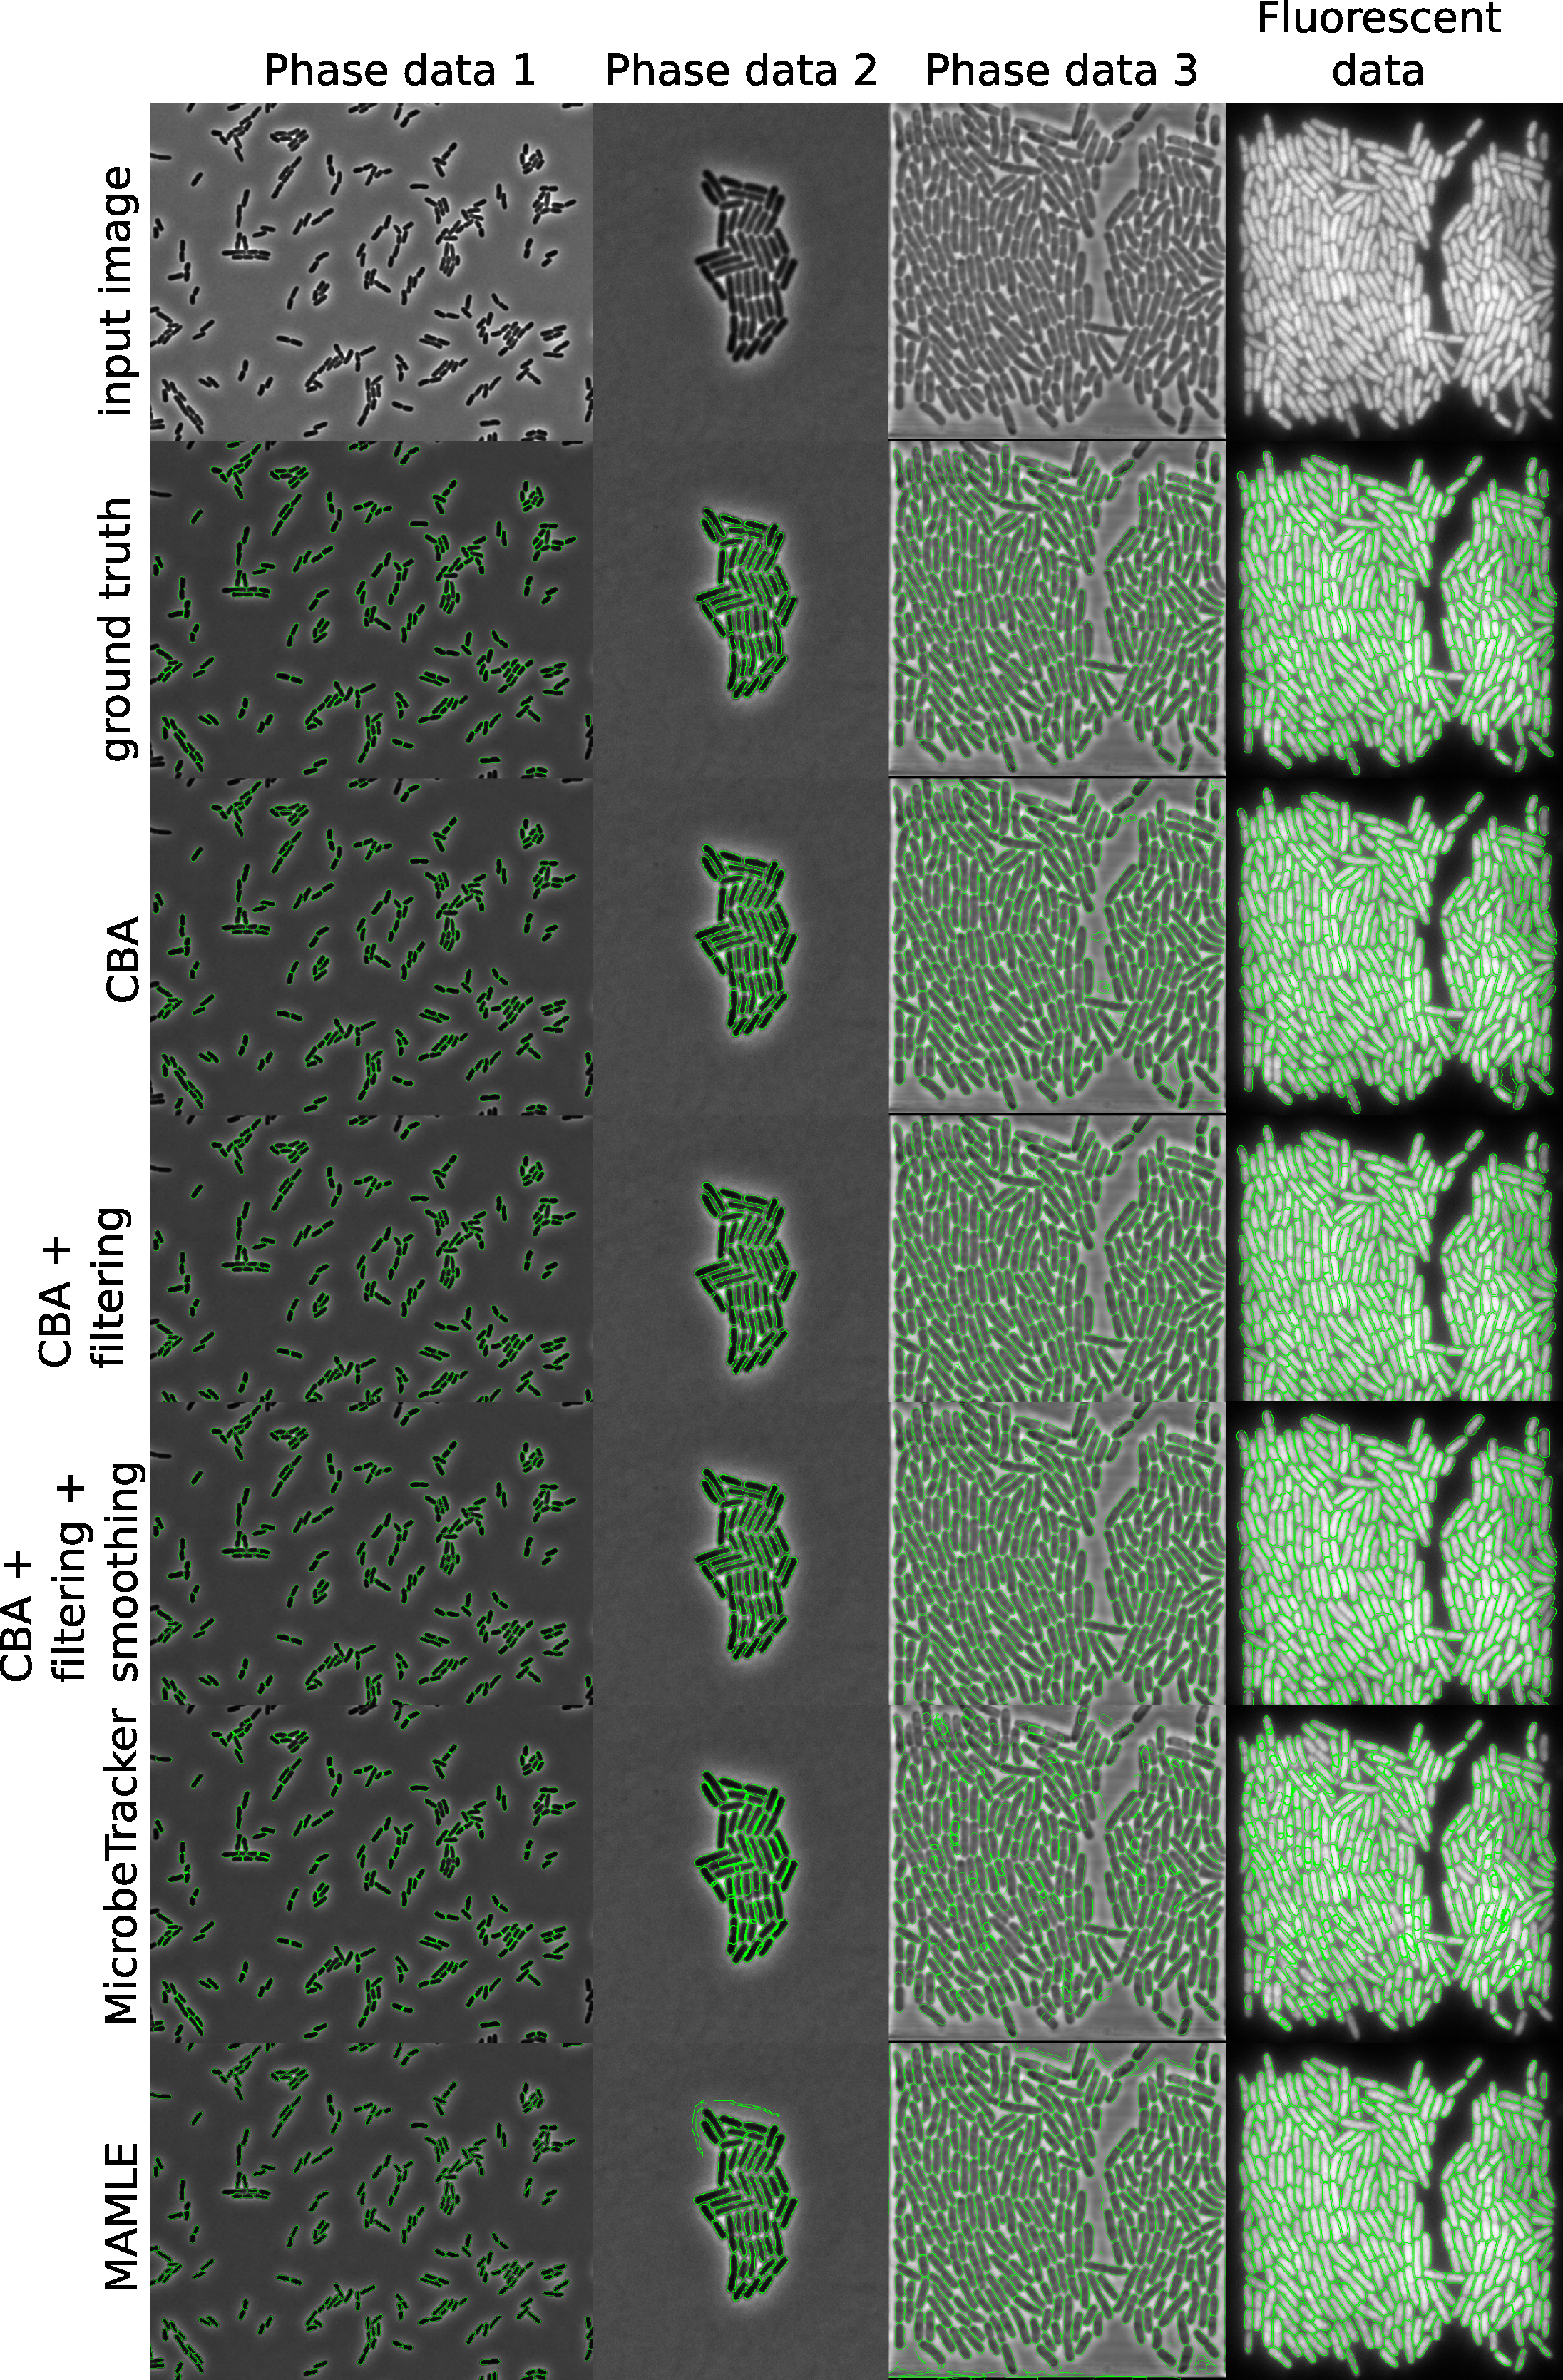
\includegraphics[width=7.5cm]{fig3edrgb.png}			
		
		\caption{Segmentation results: phase data $1$ is from the \textit{MicrobeTracker} dataset, phase data $2$ from \textit{Schnitzcells} dataset, phase data $3$ and fluorescent data from our dataset. Phase data 1 and 2 are from experiments on agarose pads whereas phase data 3 and fluorescent data are from a growth medium in a PDMS device.}\label{fig:segcompare}
	\end{center}
\end{figure}


\begin{figure}[h]
	\begin{center}
		
		\includegraphics[width=7.5cm]{fig4ed.png}					
		\caption{Zoomed-in versions of selected regions from figure \ref{fig:segcompare}.}\label{fig:segcomparezoom}
	\end{center}
\end{figure}

The Figure \ref{fig:areadistribution} shows that the area distributions are maintained prior to evaluation of segmentation results as discussed in the methods section. Evaluation results are shown in Figure \ref{fig:fscorecumul}. To summarize the comparison of the segmentation algorithms, we tested a range of thresholds on the F-score to quantify what proportion of the cells was correctly identified at different requirements on achieved F-score. We finally set a threshold at $0.8$ for the F-score, representing a decent bacterial outline, and found the percentage of bacterial cells that have an F-score greater than $0.8$ for each tested algorithm. The results show that using CBA, $87\%$ of the cells fall above this threshold, as compared to $48\%$ of the cells when using  \textit{MicrobeTracker}, and $83\%$ when using \textit{MAMLE} on the phase contrast image from our dataset (phase data 1). For our fluorescence microscopy image (fluorescent data), the value is $87\%$ for CBA while it is $46\%$ for \textit{MicrobeTracker} and $76\%$ for \textit{MAMLE}. For the \textit{MicrobeTracker} phase contrast image (phase data 1), the values are $91\%$ for CBA while $82\%$ for \textit{MicrobeTracker} and $90\%$ for \textit{MAMLE}. For the \textit{Schnitzcells} phase contrast image (phase data 2), the values are $78\%$ for CBA, $46\%$ for \textit{MicrobeTracker} and $85\%$ for \textit{MAMLE}.

The performance of CBA was only marginally improved when adding intensity based filtering and contour smoothing. However, the contour smoothing may be necessary for applications where exact edge positioning is crucial, e.g., when relating the position of sub-cellular signals to the cell edge.

\begin{figure}[!h]
	\centering
	\begin{tabular}{c c }
		\includegraphics[width=0.45\linewidth]{phasdat1areadist.png} & \includegraphics[width=0.45\linewidth]{phasdat2areadist.png} \\
		(a) & (b)\\
		\includegraphics[width=0.45\linewidth]{phasdat3areadist.png}&\includegraphics[width=0.45\linewidth]{fluoareadist.png}\\
		(c) & (d)
	\end{tabular}
	\caption{ Area distribution of segmented cells for a) phase data 1, b) phase data 2 c) phase data 3 and d) fluorescent data. }
	\label{fig:areadistribution}
	
\end{figure}

\begin{figure}[!h]
	\centering
	\begin{tabular}{c c }
		\includegraphics[height=3cm]{phasdat1fscorecumul.png} & \includegraphics[height=3cm]{phasdat2fscorecumul.png} \\
		(a) & (b)\\
		\includegraphics[height=3cm]{phasdat3fscorecumul.png} &
		\includegraphics[height=3cm]{fluofscorecumul.png}\\
		(c) & (d)
	\end{tabular}
	\caption{Cumulative \% of cells above the particular F-score for a) phase data 1, b) phase data 2, c) phase data 3 and (d) fluorescent data }
	\label{fig:fscorecumul}
	
\end{figure}


%% 


\subsection{Run Time Evaluation}
Our algorithm, CBA, was implemented in Python as a multithreaded program. We compared the execution speed of the methods on the four datasets. The time taken by each method on the four datasets is shown in figure \ref{fig:timing}. The experimental results show that the execution speed depends on the number of cells present in the image. It was found that our method, CBA, is an order of magnitude faster than the state-of-the-art methods. The results show that CBA is $10$ times faster than \textit{MicrobeTracker} and $8$ times faster than \textit{MAMLE} on average. We performed the speed evaluation on a laptop with a 2.7GHz i7 processor and 16GB RAM running on Windows 7.

\begin{figure}[h]
	\begin{center}
		
		\includegraphics[width=7.5cm]{timingrgb.png}					
		\caption{Execution times of \textit{MicrobeTracker}, \textit{MAMLE} and CBA on four datasets.}
		\label{fig:timing}
	\end{center}
\end{figure}
\subsection{Tracking Results}
To further evaluate the usability of the segmentation results produced by our proposed method, we tested its performance on a large time-lapse experiment. We applied our segmentation algorithm to time-lapse images from a dataset comprising $500$ images with approximately $250$ cells per image. $500$ frames correspond to $250$ min in real time. Cell tracking was done using the Viterbi algorithm as described in the Methods section, and we obtain a total of $10259$ tracks. The tracks were then subjected to filtering to extract candidate tracks. The track analysis stage found $1529$ tracks satisfying the criteria of having cell division at the beginning and also at the end. Since we consider cell division at the start and end of the track, essentially all tracks including the first or last $30$ min are discarded. All the $1529$ tracks were sorted in increasing order based on RANSAC fit error, as shown by the dashed line in figure \ref{fig:correcttrack} (note the logarithmic scale on the fit error). We further searched for and corrected segmentation errors in the tracks. The solid line shows the improved result, where a total of $1238$ tracks fell below the $3$ pixel error threshold prior to track correction, and $1274$ fell below the threshold afterwards.  In frames $100$ to $400$ $40\% $ of the identified cells are assigned to a track. 

\begin{figure}[h]
	\begin{center}
		
		\includegraphics[width=7.5cm]{correcttrack2.png}					
		\caption{RANSAC fit error of the major axis length in cell tracks, for the original segmentation and the error corrected segmentation, shown in logarithmic scale.}
		\label{fig:correcttrack}
	\end{center}
\end{figure}

\subsection{Comparison of Growth Rate at Different Treatments}
The second experiment included in this work was aimed at testing if the proposed method could be used to find differences in the growth rate of \textit{E. coli} cells in different media. The first dataset was obtained from \textit{E. coli} cells using glycerol as medium and the second dataset was obtained using glucose as medium. We wanted to know how fast the cells grow and divide in these two media. We found that the growth rate measured as the slope of the RANSAC fitted line was $1.2 \times 10^{-2} \pm 2.1 \times 10^{-3}$ pixels/frame in logarithmic scale (mean $\pm$ standard deviation) for cells in glucose (red) and $9.2 \times 10^{-3} \pm 1.5 \times 10^{-3}$ pixels/frame in logarithmic scale for cells in glycerol (blue). There are some cells that grow faster in glycerol and cells that grow slower in glucose as can be seen in figure \ref{fig:growthrate}.

\begin{figure}[!h]
	\centering
	\begin{tabular}{c c }
	\includegraphics[width=0.45\linewidth]{growthrateed.png} & \includegraphics[width=0.45\linewidth]{histoed.png} \\
	(a) & (b)\\
	 \includegraphics[width=0.45\linewidth]{lineagebothed.png}&\\
	 (c) &
	\end{tabular}
	\caption{Comparison of growth rates: a) Change in major axis length over time for two datasets with cells in glucose (red) and glycerol (blue). b) Histogram of slope found by RANSAC line fit for two datasets. (c) A sample lineage of  cells grown in glucose(raw data in red and RANSAC in yellow) and glycerol(raw data in blue and RANSAC in green). }
	\label{fig:growthrate}
	
\end{figure}


\section{Conclusions and Future Work}
In this work, we developed a fast and robust \textit{E. coli} cell segmentation method that can be used as input for tracking cells in time-lapse microscopy images. We also showed that our method works better than the state-of-the-art methods both in terms of accuracy and speed. The parameters required to tune for different datasets are few and depend only on the size of cells present in the input image. To show the usability of our method on actual biological datasets, we did segmentation and tracking on two different datasets and found the growth rates of the cells and their variability. This clearly shows that the proposed method has the potential to be used for a wide variety of experiments involving \textit{E. coli} cells. In the future, we would like to speed up the processing further approaching the speed of the data acquisition.




% An example of a floating figure using the graphicx package.
% Note that \label must occur AFTER (or within) \caption.
% For figures, \caption should occur after the \includegraphics.
% Note that IEEEtran v1.7 and later has special internal code that
% is designed to preserve the operation of \label within \caption
% even when the captionsoff option is in effect. However, because
% of issues like this, it may be the safest practice to put all your
% \label just after \caption rather than within \caption{}.
%
% Reminder: the "draftcls" or "draftclsnofoot", not "draft", class
% option should be used if it is desired that the figures are to be
% displayed while in draft mode.
%
%\begin{figure}[!t]
%\centering
%\includegraphics[width=2.5in]{myfigure}
% where an .eps filename suffix will be assumed under latex, 
% and a .pdf suffix will be assumed for pdflatex; or what has been declared
% via \DeclareGraphicsExtensions.
%\caption{Simulation results for the network.}
%\label{fig_sim}
%\end{figure}

% Note that IEEE typically puts floats only at the top, even when this
% results in a large percentage of a column being occupied by floats.


% An example of a double column floating figure using two subfigures.
% (The subfig.sty package must be loaded for this to work.)
% The subfigure \label commands are set within each subfloat command,
% and the \label for the overall figure must come after \caption.
% \hfil is used as a separator to get equal spacing.
% Watch out that the combined width of all the subfigures on a 
% line do not exceed the text width or a line break will occur.
%
%\begin{figure*}[!t]
%\centering
%\subfloat[Case I]{\includegraphics[width=2.5in]{box}%
%\label{fig_first_case}}
%\hfil
%\subfloat[Case II]{\includegraphics[width=2.5in]{box}%
%\label{fig_second_case}}
%\caption{Simulation results for the network.}
%\label{fig_sim}
%\end{figure*}
%
% Note that often IEEE papers with subfigures do not employ subfigure
% captions (using the optional argument to \subfloat[]), but instead will
% reference/describe all of them (a), (b), etc., within the main caption.
% Be aware that for subfig.sty to generate the (a), (b), etc., subfigure
% labels, the optional argument to \subfloat must be present. If a
% subcaption is not desired, just leave its contents blank,
% e.g., \subfloat[].


% An example of a floating table. Note that, for IEEE style tables, the
% \caption command should come BEFORE the table and, given that table
% captions serve much like titles, are usually capitalized except for words
% such as a, an, and, as, at, but, by, for, in, nor, of, on, or, the, to
% and up, which are usually not capitalized unless they are the first or
% last word of the caption. Table text will default to \footnotesize as
% IEEE normally uses this smaller font for tables.
% The \label must come after \caption as always.
%
%\begin{table}[!t]
%% increase table row spacing, adjust to taste
%\renewcommand{\arraystretch}{1.3}
% if using array.sty, it might be a good idea to tweak the value of
% \extrarowheight as needed to properly center the text within the cells
%\caption{An Example of a Table}
%\label{table_example}
%\centering
%% Some packages, such as MDW tools, offer better commands for making tables
%% than the plain LaTeX2e tabular which is used here.
%\begin{tabular}{|c||c|}
%\hline
%One & Two\\
%\hline
%Three & Four\\
%\hline
%\end{tabular}
%\end{table}


% Note that the IEEE does not put floats in the very first column
% - or typically anywhere on the first page for that matter. Also,
% in-text middle ("here") positioning is typically not used, but it
% is allowed and encouraged for Computer Society conferences (but
% not Computer Society journals). Most IEEE journals/conferences use
% top floats exclusively. 
% Note that, LaTeX2e, unlike IEEE journals/conferences, places
% footnotes above bottom floats. This can be corrected via the
% \fnbelowfloat command of the stfloats package.







% if have a single appendix:
%\appendix[Proof of the Zonklar Equations]
% or
%\appendix  % for no appendix heading
% do not use \section anymore after \appendix, only \section*
% is possibly needed

% use appendices with more than one appendix
% then use \section to start each appendix
% you must declare a \section before using any
% \subsection or using \label (\appendices by itself
% starts a section numbered zero.)
%




% use section* for acknowledgment
\section*{Acknowledgment}


The authors would like to thank the financial support from the Swedish research council, grant 2012-4968, and Swedish strategic research program, eSSENCE, to Carolina W\"ahlby.

%\newpage
% Can use something like this to put references on a page
% by themselves when using endfloat and the captionsoff option.
%\ifCLASSOPTIONcaptionsoff
%  \newpage
%\fi



% trigger a \newpage just before the given reference
% number - used to balance the columns on the last page
% adjust value as needed - may need to be readjusted if
% the document is modified later
%\IEEEtriggeratref{8}
% The "triggered" command can be changed if desired:
%\IEEEtriggercmd{\enlargethispage{-5in}}

% references section

% can use a bibliography generated by BibTeX as a .bbl file
% BibTeX documentation can be easily obtained at:
% http://www.ctan.org/tex-archive/biblio/bibtex/contrib/doc/
% The IEEEtran BibTeX style support page is at:
% http://www.michaelshell.org/tex/ieeetran/bibtex/
\bibliographystyle{IEEEtran}
\bibliography{sample}

\end{document}


